\documentclass[a4paper]{article}

%% Language and font encodings
\usepackage[english]{babel}
\usepackage[utf8]{inputenc}
\usepackage[T1]{fontenc}
\usepackage{authblk}
\usepackage[export]{adjustbox}
\usepackage{booktabs}
\usepackage{ae,aecompl}
%% Sets page size and margins
\usepackage[a4paper,top=3cm,bottom=2cm,left=3cm,right=3cm,marginparwidth=1.75cm]{geometry}

%% Useful packages
\usepackage{pgfplots}
\pgfplotsset{compat=1.12}
\usepackage[group-separator={,}]{siunitx}
\usepackage{amsmath}
\usepackage{wrapfig}
\usepackage{amsthm}
\usetikzlibrary{arrows,automata}
\usepackage{algpseudocode}
\usepackage{graphicx}
\usepackage{algorithm}
\usepackage{breqn}
\usepackage{algpseudocode}
\usepackage{float}
\usepackage{tikz}
\usepackage{pifont}% http://ctan.org/pkg/pifont
\newcommand{\cmark}{\ding{51}}%
\newcommand{\xmark}{\ding{55}}%
\usepackage{eufrak}
\usepackage{caption}
\usepackage{subcaption}
\usepackage{listings}
\usepackage[toc,page]{appendix}
\usepackage{color}
\definecolor{lightgray}{rgb}{.9,.9,.9}
\definecolor{darkgray}{rgb}{.4,.4,.4}
\definecolor{purple}{rgb}{0.65, 0.12, 0.82}
\floatname{algorithm}{Procedure}
\renewcommand{\algorithmicrequire}{\textbf{Input:}}
\renewcommand{\algorithmicensure}{\textbf{Output:}}

\lstdefinelanguage{JavaScript}{
	keywords={typeof, contract, struct, new, true, false, catch, function, return, null, catch, switch, var, if, in, while, do, else, case, break},
	keywordstyle=\color{blue}\bfseries,
	ndkeywords={class, export, boolean, throw, implements, import, this},
	ndkeywordstyle=\color{darkgray}\bfseries,
	identifierstyle=\color{black},
	sensitive=false,
	comment=[l]{//},
	morecomment=[s]{/*}{*/},
	commentstyle=\color{purple}\ttfamily,
	stringstyle=\color{red}\ttfamily,
	morestring=[b]',
	morestring=[b]"
}

\lstset{
	language=JavaScript,
	backgroundcolor=\color{lightgray},
	extendedchars=true,
	basicstyle=\footnotesize\ttfamily,
	showstringspaces=false,
	showspaces=false,
	numbers=left,
	numberstyle=\footnotesize,
	numbersep=9pt,
	tabsize=2,
	breaklines=true,
	showtabs=false,
	captionpos=b
}

\usepackage{graphicx}
\usepackage[
n,
operators,
advantage,
sets,
adversary,
landau,
probability,
notions,	
logic,
ff,
mm,
primitives,
events,
complexity,
asymptotics,
keys]{cryptocode}
\usepackage[colorinlistoftodos]{todonotes}
\usepackage[colorlinks=true, allcolors=blue]{hyperref}

\theoremstyle{definition}
\newtheorem{definition}{Definition}[section]

\newcommand{\Mod}[1]{\ (\mathrm{mod}\ #1)}

\def\bitcoinA{%
	\leavevmode
	\vtop{\offinterlineskip %\bfseries
		\setbox0=\hbox{B}%
		\setbox2=\hbox to\wd0{\hfil\hskip-.03em
			\vrule height .3ex width .15ex\hskip .08em
			\vrule height .3ex width .15ex\hfil}
		\vbox{\copy2\box0}\box2}}

\DeclareMathOperator{\EX}{\mathbb{E}}% expected value
\providecommand{\keywords}[1]{\textbf{\textit{Keywords:}} #1}

\renewcommand{\lstlistingname}{Figure}% Listing -> Algorithm
\renewcommand{\lstlistlistingname}{List of \lstlistingname s}% List of Listings -> List of Algorithms

\newcommand{\smallsim}{\smallsym{\mathrel}{\sim}}

\makeatletter
\newcommand{\smallsym}[2]{#1{\mathpalette\make@small@sym{#2}}}
\newcommand{\make@small@sym}[2]{%
	\vcenter{\hbox{$\m@th\downgrade@style#1#2$}}%
}
\newcommand{\downgrade@style}[1]{%
	\ifx#1\displaystyle\scriptstyle\else
	\ifx#1\textstyle\scriptstyle\else
	\scriptscriptstyle
	\fi\fi
}
\makeatother


\title{Dynamic Network Analysis of Bitcoin's Lightning Network}
\author[1]{Ferenc Béres}
\author[2]{István András Seres}
\author[3]{Claas Brüß}
\author[4]{András Benczúr}
\affil[1,4]{MTA SZTAKI}
\affil[2]{Department of Computer Algebra, Eötvös Loránd University}
\affil[3]{Technise Universität München}
\begin{document}
\maketitle

\begin{abstract}
 
\end{abstract}
\keywords{Bitcoin, Lightning Network, Temporal Network Analysis, Simulation, Network Topology, Payment Channel Network}

%% Pisti
\section{Introduction}
\subsection{Related work}

\textbf{Our contribution:}

\section{Background}
\subsection{Network properties}
Let $E(t)$ and $N(t)$ denote the number of edges and nodes at time $t$ respectively.
\subsection{Bitcoin and Lightning Network}

\section{Data}
\section{Experiments}
\subsection{Simulating transactions on LN}
\subsection{LN's evolution}
\subsubsection{Macroscopic evolution}
Ever since LN had been launched its popularity steadily grew, causing its average degree increasing over time. In \cite{leskovec2008dynamics} it was shown that densification of real networks follow power-law distribution, i.e.: 
\begin{equation}
	E(t) \propto N(t)^{a},
\end{equation} \label{rel:dpl}
where we call $a$ the power law densification exponent, where  $1\leq a \leq 2$. If $a=1$, then average degree of the network is constant over time, on the other hand if $a=2$, the network is an extremely dense graph, where each node has, on average, edges to a constant fraction of all nodes \cite{leskovec2008dynamics}. We found that LN is no exception to the DPL rule (\ref{rel:dpl}).

\begin{figure}[H]
	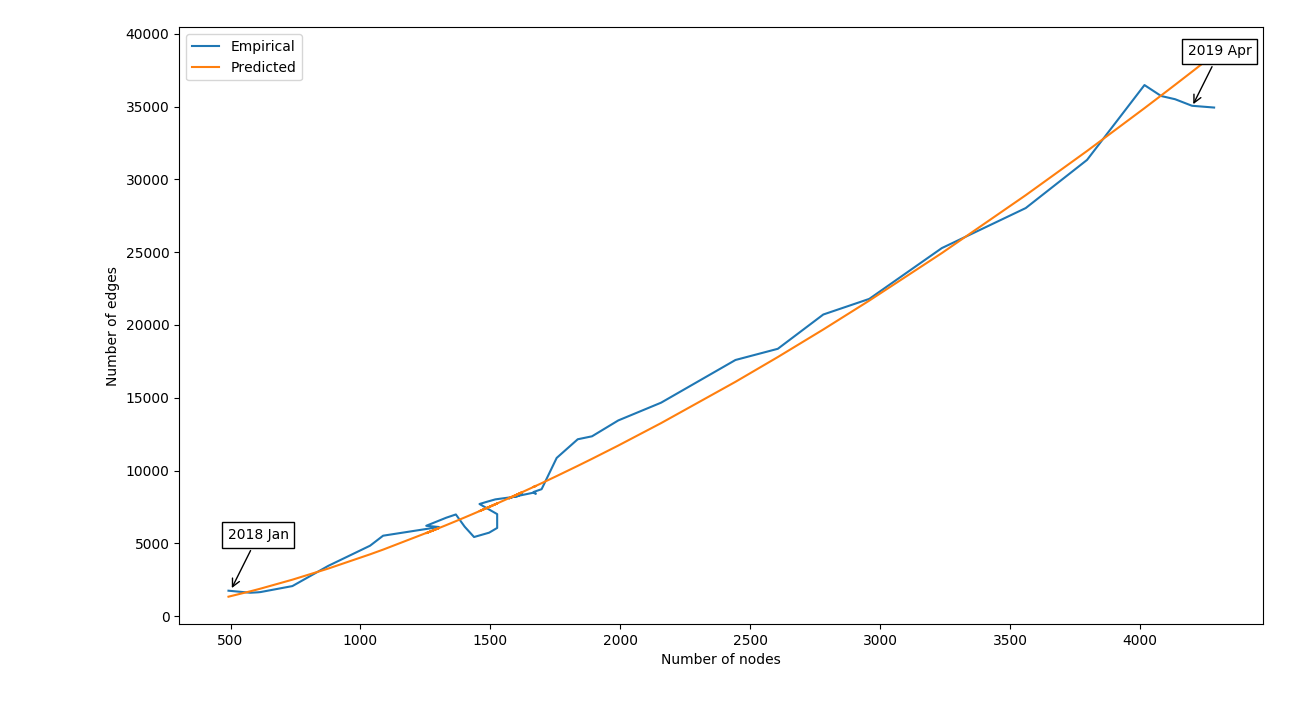
\includegraphics[width=\textwidth]{densificationPowerLaw.png}
	\label{fig:densification}
	\caption{LN follows the Densification Power Law relation with exponent $a=1.55634117$. Goodness-of-fit: $R^2=0.98$.  }
\end{figure}

\subsubsection{Densification of LN}
\subsubsection{Link prediction}
\section{Results}
\section{Acknowledgements}
Antoine and Altangent Labs

\bibliographystyle{plain}
\bibliography{sample}

\end{document}
